\documentclass[twoside,11pt]{article}
\usepackage[preprint]{jmlr2e}
\usepackage{lmodern}
\usepackage{amsmath,mathtools,booktabs,longtable,array,microtype,enumitem,xcolor}
\hypersetup{hidelinks,pdftitle={Kernel Affine Hull Features for Natural Forecasting: Accuracy, Computational Cost, and Predicting Benefit},pdfauthor={Mohit Kumar and Somayeh Kargaran}}
\newcommand{\R}{\mathbb{R}}
\newcommand{\E}{\mathbb{E}}
\newcommand{\Var}{\operatorname{Var}}
\newcommand{\MSE}{\operatorname{MSE}}
\allowdisplaybreaks
\ShortHeadings{KAHM Features for Natural Forecasting}{Kumar and Kargaran}
\firstpageno{1}
\begin{document}
\title{Kernel Affine Hull Features for Natural Forecasting:\\
Accuracy, Computational Cost, and Predicting Benefit\thanks{Research draft for author review; not submitted. AI tools assisted with protocol development, implementation, validation, analysis, and writing. The authors must independently verify and approve the final submission.}}
\author{\name Mohit Kumar \AND \name Somayeh Kargaran}
\maketitle
\begin{abstract}%
Kernel Affine Hull Machine (KAHM) features encode local reconstruction
geometry, but their forecasting value depends on the target, decoder, and
cost of fitting and selecting a model. We evaluate this dependence on eight
original natural-data source families, separating four development families
from four reserved confirmation families. Twenty-six series, two
context--horizon settings, two capacities, and two seeds yield 208 task runs.
Comparators include independently fitted affine and locality features,
raw-history kernel and linear models, and conventional forecasting controls.
Costs include preprocessing, validation search, refitting, prediction, and
selector dependencies. On confirmation sources, raw-history-plus-KAHM has
4.26\% higher source-balanced scaled mean-squared error than the matched
raw-history kernel predictor at 2.30 times its warm-library pipeline cost;
raw ridge has lower aggregate error than either. A diagnostic frozen before confirmation
uses metadata and a cheap validation probe to predict KAHM benefit. Adding
two geometric features changes none of its 80 confirmation decisions and
slightly worsens log-benefit prediction error. Saved forecasts independently
reproduce all 2,496 task--method losses. These bounded results identify
limitations of the tested KAHM forecasting procedure and usefulness
diagnostic; they do not establish a general KAHM advantage or impossibility
of a stronger future criterion.

\end{abstract}
\begin{keywords}
kernel affine hull machines, forecasting, local representations, algorithm selection, computational cost
\end{keywords}

\section{Introduction}\label{sec:introduction}
Local reconstruction geometry can provide features for a prediction problem,
but reconstruction quality alone does not establish their predictive usefulness.
The forecasting target, the code supplied to the decoder, regularization, and
the cost of obtaining the fitted predictor all matter. Kernel Affine Hull
Machines (KAHMs) provide a concrete setting in which to examine these questions:
their local covariance kernels and normalized reconstruction weights induce
nonlinear affinity coordinates, which can be augmented with positions in local
principal subspaces \citep{Kumar2024KAHM}. A practical forecasting claim requires
evidence about the complete fitted procedure, including the circumstances in
which an ordinary alternative should be preferred.

An archived precursor study motivated the present investigation by separating
reconstruction, score encoding, local positional information, and decoder
capacity. Its controlled branch example showed that an accurate affine
reconstructor can have an uninformative residual code, while explicit local
coordinates or a locality-aware affine gate repair much of that limitation.
A fresh-sample capacity experiment found conditional KAHM gains on Van der Pol
and unfavorable or unresolved comparisons on other synthetic laws. Those
observations motivate a test on independent natural sources; they do not supply
that test. The precursor manuscript, software, and numerical archive remain
unchanged at repository commit \texttt{a67c4019}. Appendix~\ref{app:checkpoint}
records the relationship between the two research stages.

The question addressed here is whether KAHM features provide useful forecasting
accuracy at their complete computational cost, and whether a reduced-capacity
historical diagnostic can anticipate their benefit on a reserved source family.
We examine this question in a bounded, explicitly specified experiment. Four
original source families supply development outcomes, and four different source
families supply confirmation outcomes after the diagnostic has been frozen.
The study uses 26 series and two context--horizon settings per series. Two
capacity settings and two fitting seeds yield 208 task runs, but the units of
transfer evidence remain the original source families.

Three design choices support a more specific interpretation. First, we compare
KAHM local features with independently fitted affine and locality-aware
alternatives, both with and without the complete raw history. Raw augmentation
makes information retention explicit and places the question on finite-decoder
behavior. Second, we account for preprocessing, representation learning,
validation search, final refitting, forecasting, and the computations required
by a selector. The regularization search reuses features within each method;
it does not subsidize a competing method with a shared KAHM fit. Third, the
diagnostic tests a specified increment: whether two geometric measurements add
useful information beyond historical metadata and a paid validation probe.
Feature-based forecasting selection already has substantial precedents
\citep{Prudencio2004MetaLearning,MonteroManso2020FFORMA,Talagala2022FFORMPP,Talagala2023FFORMS}.
Our experiment evaluates that increment for the declared KAHM comparison.

The confirmation findings do not support broad adoption of the tested KAHM
augmentation. Its source-balanced scaled MSE is 0.8419, compared with
0.8075 for the matched raw-history RBF predictor and 0.7798 for raw ridge.
Its measured warm-library pipeline cost is 0.3874 seconds per weighted task,
compared with 0.1688 seconds for raw RBF. The augmentation improves on raw
RBF in one of the four confirmation family means, where raw ridge is also
better. Differences from raw-plus-affine and raw-plus-locality are small
and mixed across families. These findings contrast with a favorable
development average that is dominated by one macroeconomic source.

The frozen usefulness diagnostic also has a specific negative result.
Adding geometric measurements to metadata and a validation probe changes
none of its 80 confirmation choices. Both variants obtain scaled MSE
0.8071, essentially the raw predictor's 0.8075, while costing about
0.3309 seconds. Geometry slightly worsens estimated log-benefit error.
These observations support evaluating a representation together with its
decoder, strong structural controls, complete computational dependencies,
and source-transfer evidence. They provide no validated geometric rule
for deciding when this KAHM augmentation will be beneficial.


The contribution is an auditable assessment of accuracy, cost, and usefulness
prediction for this collection of procedures and sources. It includes the
frozen task registry, measured computational dependencies, saved forecasts,
independent loss reconstruction, and unsuccessful comparisons. The experiment
does not estimate a universal KAHM advantage, establish a forecasting
state of the art, or turn repeated windows and seeds into independent domains.

\section{Related work}
\label{sec:related}

\paragraph{Reconstruction and local coordinates.}
Kernel affine hull machines (KAHMs) were introduced for geometrically informed
classification, including a differential-privacy application
\citep{Kumar2024KAHM}. We adapt their reconstruction operators to form
unsupervised gates on forecasting histories and compare them with locality
and affine-projection controls. Local coordinate coding already connects
localized representations to approximation of smooth prediction functions
\citep{Yu2009LCC}. Local tangent coding augments coding weights with weighted
displacements along local tangent directions \citep{YuZhang2010LTC}; our gated
local coordinates use this established architectural idea. The empirical
question is whether KAHM-derived gates improve forecasting within the stated
architecture and resource regimes. Classification results for the original
KAHMs and approximation results for local coding concern their own tasks
and assumptions; they do not establish the outcome of this comparison.

\paragraph{Target relevance and finite prediction procedures.}
Supervised dimension reduction explicitly seeks representations that preserve
the relationship between an input and its response \citep{Fukumizu2004SDR}.
This highlights why a representation's reconstruction quality alone does
not determine its forecasting value. Our raw-input augmentation retains the
original history, while changing the coordinates available to a particular
fitted predictor. Its finite-sample performance can therefore change through
approximation, estimation or regularization without a change in the
information contained in that history. We use finite Nystr\"om kernel
features \citep{Williams2001Nystrom}, so the comparison concerns specified
fitting procedures. Equal requested landmark counts after different feature
maps do not imply identical prediction classes, realized ranks or computation.
The capacity caps and measured costs make these distinctions explicit.

\paragraph{Forecast selection and performance prediction.}
Learning which forecasting method suits a series is an established problem.
\citet{Prudencio2004MetaLearning} studied both learned selection between
forecasting models and model ranking. FFORMA learns forecast-combination
weights from time-series features \citep{MonteroManso2020FFORMA}.
FFORMPP predicts forecasting errors from historical-series features and
uses those predictions for selection or combination
\citep{Talagala2022FFORMPP}; FFORMS learns a feature-based mapping to a
selected forecasting model \citep{Talagala2023FFORMS}. These works also
motivate attention to computation and the representativeness of the data
used to train a selector. Here a deliberately small, fixed ridge diagnostic
predicts the relative benefit of appending KAHM local features to a raw-history
kernel predictor. The main question is the incremental value of geometric
features beyond metadata and a fixed validation probe. Performance comparisons
apply to the implemented candidates and selectors. Four development families
and four reserved families support a bounded examination of this question,
with substantial limits on transfer to additional domains.

\paragraph{Cheap probes and the cost of choosing a method.}
Landmarking characterizes a learning task using the measured performance of
inexpensive learners \citep{Pfahringer2000Landmarking}. Our cheap validation
probe follows this general principle: it supplies evidence about the target
that input-only geometric features do not directly measure. We retain both
metadata-only and probe-augmented diagnostic controls, and charge the probe
and geometry computation even when the eventual decision selects the raw
predictor. The accounting also charges all searches needed by a validation
selector, followed by the chosen candidate's refit and forecast. Offline
diagnostic fitting and per-task inference are reported separately. This
evaluates the computational consequences of the declared decision rules;
the learned rule, the use of probes and the general accuracy--cost tradeoff
are established ideas.

\paragraph{Forecast evaluation and source separation.}
Reusing a finite model-selection criterion for evaluation can produce
optimistic conclusions \citep{Cawley2010Selection}. Forecasting adds concerns
about temporal information, scaling, appropriate simple baselines and
dependent errors \citep{Hewamalage2023Evaluation}. We use chronological
training, validation and test blocks; the separate development/confirmation
division concerns the original data sources from which those tasks arise.
The Monash archive supplies datasets from varied domains and documented
baseline evaluations \citep{Godahewa2021Monash}. We use pinned snapshots and
keep derived series, horizons, capacities and seeds within their source
families for aggregation. Diagnostic features and regularization are fixed
before development outcomes, and fitted diagnostics are frozen before
confirmation evaluation. The small, deliberately chosen family collection
supports descriptive source-level comparisons, not population-wide
confidence claims. This is a historical forecasting study; it does not
establish real-time deployment performance or performance under future
changes in data availability.

\section{Representations and fitted forecasting rules}
\label{sec:nf-methods}

A history $x\in\mathbb R^d$ contains the observations available at a forecast
origin; its response $y\in\mathbb R^H$ contains the next $H$ observations.
For the univariate tasks below, the input dimension $d$ equals the history length $L$.
We fit direct multioutput regressors to historical pairs
$\{(x_i,y_i)\}_{i=1}^n$.  The construction below specifies which part of the
regressor uses KAHM geometry.  It does not assume that overlapping forecasting
windows are independent.  All input transformations, reference sets, and
decoder bases are fitted on the training portion of each fit.

\subsection{Shared reference geometry}
\label{sec:nf-reference-geometry}

Write $z(x)=D^{-1}(x-\bar x)$, where $\bar x$ and the diagonal scales $D$ are
training means and population standard deviations.  A standard deviation at
most $10^{-12}$ is replaced by one.  Thus this transformation retains every
raw coordinate, including coordinates constant in the observed training set.
Three independently seeded $k$-means partitions, with $k\in\{2,4,8\}$, use
the same seeded subset of at most 512 training histories.  Each partition has
five initializations and at most 150 iterations.  Each cluster supplies at
most 24 references sampled without replacement; all its rows are used if
there are fewer.  For a common seed and training set, the alternative gates
use identical partition and reference-selection rules.  They are nevertheless
fitted as separate computational pipelines.

Index the 14 local models by $c$, with the partition blocks denoted
$\mathcal C_b$.  Let
$Q_c=[q_{c1},\ldots,q_{cm_c}]\in\mathbb R^{d\times m_c}$ contain the
training-standardized references, stored after the inherited float32
conversion, and let $\mu_c=m_c^{-1}Q_c\mathbf 1$.
The orthonormal columns of $P_c\in\mathbb R^{d\times r_c}$ are leading
eigenvectors of the centered reference covariance.  The requested rank is
$\min(2,d-1,m_c-1)$; only eigenvalues above double-precision machine epsilon
are retained.  The inherited implementation further reduces a rank greater
than one if the smallest projected coordinate range is below $10^{-3}$.
A reference set with no usable direction has $r_c=0$ and uses its center as
its reconstruction.  Other numerical failures remain recorded failures.

The affine reconstruction and centered local coordinates are
\begin{equation}
 a_c(z)=\mu_c+P_cP_c^\top(z-\mu_c),
 \qquad u_c(z)=P_c^\top(z-\mu_c).
 \label{eq:nf-affine}
\end{equation}
The affine and locality controls compute these quantities without fitting or
querying any KAHM kernel.

\subsection{Reconstruction scores and local gates}
\label{sec:nf-gates}

\paragraph{KAHM reconstruction.}
Kernel Affine Hull Machines construct nonlinear reconstructions from local
kernel weights \citep{Kumar2024KAHM}.  We retain the pinned implementation's
local autoencoder, rather than asserting equivalence to an independently
optimized end-to-end KAHM learner.  For $r_c>0$, let $\Sigma_c$ be the sample
covariance of the columns of $P_c^\top Q_c$.  Its Gaussian kernel is
\begin{equation}
 k_c(z,q)=\exp\!\left\{-\frac{
  (P_c^\top(z-q))^\top\Sigma_c^{-1}P_c^\top(z-q)}{2r_c}\right\},
 \qquad (K_c)_{ij}=k_c(q_{ci},q_{cj}).
 \label{eq:nf-kahm-kernel}
\end{equation}
To specify the inherited local regularizer exactly, put
$\nu_c=\|Q_c\|_F^2/(dm_c)$ and initialize $\lambda_0=5\nu_c/2$.  Its iteration is
\begin{equation}
 B_t=(K_c+\lambda_t I)^{-1},\qquad
 \lambda_{t+1}=2\nu_c+
 \frac{\|Q_c-Q_c(K_cB_t)^\top\|_F^2}{dm_c}.
 \label{eq:nf-local-regularizer}
\end{equation}
It stops after an update of size at most $10^{-3}$ or 100 updates, and
retains the last computed $B_t$ as $B_c$.  In particular, it does not perform
an extra inverse at the newly updated $\lambda_{t+1}$.
For $k_c(z)=(k_c(z,q_{cj}))_{j=1}^{m_c}$, define
\begin{equation}
 v_c(z)=B_c^\top k_c(z),\qquad
 \widehat z_c(z)=\frac{Q_cv_c(z)}{\mathbf 1^\top v_c(z)}.
 \label{eq:nf-reconstruction}
\end{equation}
The weights may be signed.  The reconstruction is therefore not generally a
convex average.  The inherited exact-zero-denominator convention replaces
the denominator by one; that convention is an implementation choice, not
a definition of a continuous extension at a singularity.

\paragraph{Stable Gaussian evaluation.}
For queries we compute the analytic log kernel
$\ell_{cj}(z)=-\|S_cP_c^\top(z-q_{cj})\|^2/(2r_c)$, where $S_c$ is the
stored symmetric square root of the inverse covariance, and use
$\widetilde k_{cj}(z)=\exp\{\ell_{cj}(z)-\max_j\ell_{cj}(z)\}$ in
Equation~\eqref{eq:nf-reconstruction}.
In exact arithmetic, $S_c^\top S_c=\Sigma_c^{-1}$, and multiplying every
kernel entry for one query by the same positive constant cancels from the
normalized reconstruction whenever its denominator is nonzero.
This calculation avoids underflow caused solely by a large common negative
log-kernel offset.  It does not prevent signed cancellation, guarantee a
well-conditioned denominator, or guarantee equivalence at an exact zero.
The implementation retains the zero-denominator convention, records numerical
diagnostics, and rejects nonfinite outputs.  The historical mode instead
exponentiates the unshifted logs through the inherited query routine; it is
retained for equivalence checks, while this study uses the shifted evaluation.

\paragraph{Matched folding gates.}
Given either the KAHM reconstruction $\widehat z_c$ or the affine
reconstruction $a_c$, denote it by $r_c^{\mathrm{rec}}(z)$.  Define
\begin{align}
 \rho_c(z)&=1-\exp\{-\|z-r_c^{\mathrm{rec}}(z)\|\},\qquad
 \theta_c(z)=\frac1\pi\arccos\!\left(
 \operatorname{clip}_{[-1,1]}
 \frac{z^\top r_c^{\mathrm{rec}}(z)}{\|z\|\,\|r_c^{\mathrm{rec}}(z)\|}\right),
 \notag\\
 s_c(z)&=\sqrt{\{\rho_c(z)^2+\theta_c(z)^2\}/2},\qquad
 \phi_c(z)=\frac{[1-\operatorname{clip}_{[0,1]}s_c(z)+\tau]^\omega}
 {\sum_{j\in\mathcal C_b}[1-\operatorname{clip}_{[0,1]}s_j(z)+\tau]^\omega},
 \quad c\in\mathcal C_b.
 \label{eq:nf-folding-gates}
\end{align}
When either norm in the cosine denominator is zero, its cosine is set to
zero, so that $\theta_c=1/2$.  The fixed values are $\omega=16$ and
$\tau=10^{-6}$; normalization is evaluated with log-sum-exp.  The comparison
between these two gates changes the reconstruction while retaining the
score, reference geometry, and local-coordinate construction.

\paragraph{Locality control.}
The third gate uses the historical native-affine score formula, applied to
the same references.  With $\epsilon=10^{-6}$, set
\begin{align}
 t_c&=\max\!\left\{m_c^{-1}\sum_j\|q_{cj}-\mu_c\|^2,\epsilon\right\},\notag\\
 e_c&=\max\!\left\{m_c^{-1}\sum_j\|q_{cj}-a_c(q_{cj})\|^2,
                    0.05t_c,\epsilon\right\},\notag\\
 b_c(z)&=\frac{\|z-a_c(z)\|^2}{e_c}
          +0.1\frac{\|z-\mu_c\|^2}{t_c},\notag\\
 \phi_c(z)&=\frac{\exp[-b_c(z)]}
                    {\sum_{j\in\mathcal C_b}\exp[-b_j(z)]}.
 \label{eq:nf-locality-gates}
\end{align}
This distinguishes proximity to the local center from projection residual.
Here ``native'' identifies a score formula; it does not identify a separately
tuned native learning algorithm.  It supplies a non-KAHM locality alternative
to the matched folding-score comparison.

\subsection{Local codes and finite forecasting heads}
\label{sec:nf-local-features}

For each gate family $g$, concatenate all gates and gated local coordinates:
\begin{equation}
 T_g(x)=\bigl((\phi_c(z(x)))_c,
                  (\phi_c(z(x))u_c(z(x)))_c\bigr),\qquad
 T_{\mathrm{raw}+g}(x)=(z(x),T_g(x)).
 \label{eq:nf-local-code}
\end{equation}
The stored local width is $14+\sum_c r_c\leq42$; the actual width is recorded.
The raw augmentation prepends all $d$ history coordinates, with no truncation
when $d>28$.  The combination of local association and local position is
related to coordinate and tangent coding \citep{Yu2009LCC,YuZhang2010LTC};
our gates and decoder are the explicit constructions above.
The stack of $P_c^\top$ has rank at most 28.  A deficient stack alone does
not prove information loss in $T_g$, because the gates also depend on the
query.  Raw augmentation gives the simpler unconditional reconstruction
property stated below, without a rank assumption.

\paragraph{Nystr\"om plus linear basis.}
\label{sec:nf-head}
Let $v(x)$ denote $z(x)$, $T_g(x)$, or $T_{\mathrm{raw}+g}(x)$, and let
$q(x)$ be its coordinatewise training standardization.  Select $M$ training
rows without replacement as landmarks $a_1,\ldots,a_M$ in $q$-space.
The requested $M$ is 32 or 64, capped by the training size.
Set $\sigma^2$ to the median positive squared inter-landmark distance and
define
\begin{equation}
 k_\sigma(q,a)=\exp\{-\|q-a\|^2/(2\sigma^2)\},\qquad
 b(x)=\left(q(x),\;
       \operatorname{diag}(\eta_J^{-1/2})U_J^\top
                  (k_\sigma(q(x),a_j))_{j=1}^M\right).
 \label{eq:nf-nystrom}
\end{equation}
Here $U\operatorname{diag}(\eta)U^\top$ diagonalizes the landmark Gram
matrix, and $J$ retains eigenvalues exceeding
$\max(10^{-10}\eta_{\max},10^{-12})$ \citep{Williams2001Nystrom}.
Distances at most $10^{-14}$ are excluded from the bandwidth median;
if none remain the squared bandwidth is one, and in all cases it is floored
at $10^{-12}$.  The bandwidth multiplier is fixed to one.
Finally, standardize $b$ on training rows to obtain $f(x)$ and the design
$F_{i,:}=f(x_i)^\top$.  Both head standardizations replace scales below
$10^{-8}$ by one.  Raw ridge omits the Nystr\"om block and uses the same
centering and scaling convention.

For each horizon $h$, the fitted decoder solves
\begin{equation}
 \min_{\beta_h,a_h}\ \frac1n\sum_{i=1}^n
       [y_{ih}-a_h-f(x_i)^\top\beta_h]^2+\alpha\|\beta_h\|^2.
 \label{eq:nf-ridge-objective}
\end{equation}
Thus the normal equations use $F^\top F/n+\alpha I$, and the intercept is
unpenalized.  Internally, targets are standardized using training statistics
and transformed back after prediction.  For fixed $\alpha$, linearity makes
this exactly equivalent in real arithmetic to
Equation~\eqref{eq:nf-ridge-objective} in the original target units.
This is a Euclidean ridge penalty on a standardized finite basis, rather
than the canonical Gaussian RKHS norm.  Adding local features also changes
the Gaussian distances and the resulting Nystr\"om basis; the raw and
augmented nonlinear decoder classes need not be nested.

One common $\alpha$ from the ordered grid $(0.01,1,100)$ is selected by validation MSE averaged
over origins and horizons in original target units, with the first grid
entry winning ties.  Within a method, geometry, training and validation
features, basis construction, and the Gram eigensystem are computed once;
all three alphas reuse those quantities.  Different method variants share
no fitted bank or free preprocessing.  The selected configuration is then
fitted anew on the admissible pretest training data.  Search designs and
eigensystems are not retained in the serialized final model.  This gives
an explicit efficient search whose full computation can be measured.

\subsection{Information and finite-decoder risk}
\label{sec:nf-information}

The following elementary facts delimit the interpretation of the experiments.
They are established information-preservation and linear-smoother algebra,
not new KAHM approximation theorems or performance guarantees.

\begin{proposition}[Information preserved by raw augmentation]
\label{prop:nf-raw-preservation}
Condition on a fitted state $\Theta$ containing $\bar x$, positive diagonal
$D$, and a measurable, finite-valued feature map $T_g$ on the support of $X$.
Then $T_{\mathrm{raw}+g}(X)$ and $X$ generate the same information conditional
on $\Theta$.  For a square-integrable response $Y$, their conditional
expectations and optimal squared-loss Bayes risks coincide, conditional on
$\Theta$.  This statement requires neither positive gates nor a full-rank
stack of local bases.
\end{proposition}
\begin{proof}
The augmented code is a measurable function of $(X,\Theta)$, and its first
$d$ coordinates recover $X=\bar x+Dz(X)$.  Consequently
$\sigma(T_{\mathrm{raw}+g}(X),\Theta)=\sigma(X,\Theta)$.
Conditional expectation onto these equal sigma-fields, and hence the
minimum squared prediction error, is identical.
\end{proof}

This is an exact-arithmetic statement about the representation, not a
conditioning guarantee or a claim that a particular fitted decoder uses
every retained coordinate.  Empirical gains from raw augmentation must
therefore be explained through finite fitting, representation-dependent
regularization, or numerical behavior, rather than increased Bayes
information relative to the same raw input.

\begin{proposition}[Fixed-feature, fixed-alpha risk identity]
\label{prop:nf-linear-risk}
Consider one response coordinate, a fixed $\alpha>0$, and the centered
training design $F$ above.  Let $\mathcal G$ contain the training and query
inputs and the randomness used to fit their unsupervised feature map, so
$F$ and $f(x_*)$ are $\mathcal G$-measurable.  Put
\begin{equation}
 w_* = \frac{\mathbf 1}{n}
       +F(F^\top F+n\alpha I)^{-1}f(x_*).
 \label{eq:nf-smoother}
\end{equation}
Let the training response vector be $Y$, the future response be $Y_*$, and
assume their conditional second moments are finite.  Define
$\mu=\mathbb E[Y\mid\mathcal G]$,
$\mu_*=\mathbb E[Y_*\mid\mathcal G]$,
$\Sigma=\operatorname{Cov}(Y\mid\mathcal G)$,
$c=\operatorname{Cov}(Y,Y_*\mid\mathcal G)$, and
$v_*=\operatorname{Var}(Y_*\mid\mathcal G)$.  The fitted prediction is
$\widehat Y_*=w_*^\top Y$, and
\begin{equation}
 \mathbb E[(\widehat Y_*-Y_*)^2\mid\mathcal G]
   =(w_*^\top\mu-\mu_*)^2+w_*^\top\Sigma w_*+v_*-2w_*^\top c.
 \label{eq:nf-dependent-risk}
\end{equation}
\end{proposition}
\begin{proof}
Because $F^\top\mathbf 1=0$, the unpenalized intercept is $\bar Y$ and
$\widehat\beta=(F^\top F+n\alpha I)^{-1}F^\top Y$.
Substituting into $\bar Y+f(x_*)^\top\widehat\beta$ gives
Equation~\eqref{eq:nf-smoother}; the inverse target standardization cancels
as described above.  Conditional on $\mathcal G$, expand the second moment
of $w_*^\top Y-Y_*$ as its squared mean plus its variance.  The covariance
cross term is $-2w_*^\top c$, giving the identity.
\end{proof}

The identity holds without independent training responses or an independent
future response.  Overlapping windows and serial dependence can affect both
$\Sigma$ and $c$; neither may be discarded without additional assumptions.
Averaging the identity over horizons gives the corresponding average risk.
Changing geometry changes $w_*$ and can change all its bias and covariance
terms, without a universal ordering between representations.  The identity
does not automatically describe the full validation-selected procedure:
after alpha selection, the smoother depends on observed validation responses.
No generalization or selection guarantee is inferred from it.

\section{Natural-data protocol}
\label{sec:nf-protocol}

Source allocation, task roster, model grids, and analysis are fixed before
comparative outcomes.  We test matched representations, practical accuracy--cost
tradeoffs, and prospective selection on reserved families.  Specifications,
checksums, and execution freezes accompany the code as internal reproducibility
records, not externally timestamped preregistration.

\subsection{Sources and chronological tasks}
\label{sec:nf-data}

Table~\ref{tab:nf-sources} gives eight versioned Monash snapshots
\citep{Godahewa2021Monash}, chosen by provenance, application diversity, length,
and size.  Related series, channels, and aggregations share a source family
and cannot cross the boundary between development and confirmation.  Models are local to
each series, including differently dated Tourism series.  The supplement
retains the records' CC BY 4.0 licenses, versions, attribution, original-source
references, and archive hashes.

\begin{table}[t]
\caption{Fixed source allocation and forecast regimes.  ``Selected/all'' counts
series, not independent source families.  Each selected series uses both regimes
for its frequency.  $L$ is history length, $H$ forecast horizon, and $s$ the
declared seasonal period.}
\label{tab:nf-sources}
\centering\small
\setlength{\tabcolsep}{4pt}
\begin{tabular}{@{}lp{0.48\linewidth}cr@{}}
\toprule
Phase & Source snapshot & Frequency & Selected/all \\
\midrule
Development & Electricity \citep{DatasetElectricityWeekly} & weekly & 4/321 \\
 & NN5, with missing values \citep{DatasetNN5Daily} & daily & 4/111 \\
 & Tourism \citep{DatasetTourismMonthly} & monthly & 4/366 \\
 & FRED-MD \citep{DatasetFREDMD} & monthly & 4/107 \\
\midrule
Confirmation & Traffic \citep{DatasetTrafficWeekly} & weekly & 4/862 \\
 & Hospital \citep{DatasetHospitalMonthly} & monthly & 4/767 \\
 & Saugeen River flow \citep{DatasetSaugeenDaily} & daily & 1/1 \\
 & US births \citep{DatasetUSBirthsDaily} & daily & 1/1 \\
\bottomrule
\end{tabular}
\par\medskip
\begin{tabular}{@{}lccc@{}}
\toprule
Frequency & Short $(L,H)$ & Long $(L,H)$ & $s$ \\
\midrule
Monthly & $(12,3)$ & $(24,6)$ & 12 \\
Weekly & $(13,4)$ & $(26,8)$ & 52 \\
Daily & $(28,7)$ & $(56,14)$ & 7 \\
\bottomrule
\end{tabular}
\end{table}

Training-prefix eligibility requires at least 16 finite windows in each regime
and a positive training error scale.  A fixed salted hash of source and series
ID orders eligible series; we retain the first four, or all if fewer exist,
across regimes and capacities.  No later loss or availability criterion selects
replacements.  The 26 series give 52 base tasks; two capacities and seeds 17
and 43 give 208 runs: 128 development and 80 confirmation, with four source
families per phase.

For a length-$n$ series indexed from zero, let
$a=\lfloor3n/5\rfloor$ and $b=\lfloor4n/5\rfloor$.  Training, validation, and
test intervals are $[0,a)$, $[a,b)$, and $[b,n)$.  An origin $t$ is the last
observed index, with
\begin{equation}
 x_t=(y_{t-L+1},\ldots,y_t),\qquad
 y_t^+=(y_{t+1},\ldots,y_{t+H}).
 \label{eq:nf-forecast-window}
\end{equation}
The complete target interval must lie within its split; contexts may include
earlier observed values.  Stateful controls receive $t+1$, their first-future
index.  We retain raw snapshot values, including NN5 missing markers, and
discard windows with an unavailable context or target without interpolation.
Evenly spaced indices among available origins give at most 64 validation and
64 test windows, and the training cap in Table~\ref{tab:nf-capacity}.  Every
method receives the same evaluation origins.

Before outcomes, length checks reduced the proposed monthly $(48,6)$ and
weekly $(52,8)$ regimes, which yield zero Hospital and three Traffic training
windows.  The adopted long regimes yield 21 and 29, respectively.  Context
and horizon are paired, so their separate effects are not identified.
NN5 T88 at $(56,14)$ retains only seven test origins out of 146 candidates.
All task availability counts are recorded.

All candidate preprocessing is fitted on training data, and validation MSE
selects hyperparameters.  The selected pipeline is then fitted anew on all
eligible windows with targets preceding $b$, subject to its training cap.
This refit legitimately includes windows crossing the former training/validation
boundary.  Parameters are fixed thereafter; earlier realized observations may
enter later contexts or state updates.  Test outcomes never retune parameters.

\subsection{Comparators, capacity, and loss}
\label{sec:nf-comparators}

The twelve methods comprise raw ridge and raw RBF heads; affine-, locality-,
and KAHM-gated local RBF pipelines; each local pipeline augmented by the full
raw history; and seasonal naive, Holt, histogram gradient boosting, and a
one-hidden-layer MLP.  Section~\ref{sec:nf-methods} defines the feature maps and
finite RBF head.  The primary matched pair is raw RBF ($R$) versus raw-history
plus KAHM RBF ($K$).  The raw-history controls retain the inputs independently
of local-basis rank (Proposition~\ref{prop:nf-raw-preservation}).  All twelve
methods remain in the declared practical portfolio.

The geometric bank uses cluster counts $(2,4,8)$, requested rank two, at most
24 references per local model, a 512-row fitting cap, $\omega=16$, and
$\tau=10^{-6}$.  Reduced effective ranks and numerical fallbacks are recorded.
Each alternative constructs its own representation; affine/locality controls
do not fit a KAHM kernel.  Within a method, the fixed representation and head
statistics are reused across ridge penalties $\{0.01,1,100\}$; the bandwidth
multiplier is one.  Boosting/MLP regularization is chosen from $\{0.01,1\}$,
Holt selects damped or undamped trend, and seasonal naive has no tuned parameter.
These modest declared grids do not imply optimal tuning of every comparator.

\begin{table}[t]
\caption{Capacity caps.  These are limits on examples and model size, not equal
realized time budgets.  A shorter source uses its available examples.}
\label{tab:nf-capacity}
\centering\small
\setlength{\tabcolsep}{5pt}
\begin{tabular}{@{}lrrrr@{}}
\toprule
Setting & Training windows & RBF landmarks & Tree leaves/iterations & MLP width/iterations \\
\midrule
Small & 512 & 32 & 15/100 & 32/200 \\
Medium & 1,024 & 64 & 31/150 & 64/300 \\
\bottomrule
\end{tabular}
\end{table}

Seasonal naive can use its declared lag from the observed past even when it
exceeds $L$, using the last finite value for an unavailable lag and period one
before a full seasonal lag exists.  Holt fits a capped historical segment,
forward-fills only within that segment, and assimilates observations strictly
before each forecast; an absent online observation causes a state prediction
without measurement update.  Boosting and MLP fit direct multi-output forecasts
without a random internal validation split.

For recorded origins $\mathcal O$, the task score is
\begin{equation}
 \ell=\frac{1}{|\mathcal O|Hq}
       \sum_{t\in\mathcal O}\sum_{h=1}^{H}
       (\widehat y_{t+h}-y_{t+h})^2,
 \label{eq:nf-scaled-loss}
\end{equation}
Here $q$ is the seasonal-difference mean square in the uncapped initial
training prefix, requiring two finite pairs and positive finite $q$.
First differences provide the fallback; a series with neither scale is
ineligible.  This denominator remains fixed during refitting.  Raw MSE,
$q$, predictions, and origin losses are saved and independently checked.

Aggregation gives equal mass to families and then each nested dataset, series,
horizon, history, capacity, and seed.  These nested observations are not
independent source replications.  We report family outcomes, dispersion, and
leave-one-family-out sensitivity, without broad-population confidence intervals
or window-level significance claims.

\subsection{Measured pipeline and selector costs}
\label{sec:nf-costs}

Methods execute sequentially in fresh child processes with one BLAS thread
and deterministically shuffled order, limited to 120 seconds per method and
1,800 per task.  Wall and process CPU time are separate.  Each warm-library
scientific pipeline includes
data/checksum preparation, array loading, configuration fitting and validation,
selection bookkeeping, selected refitting, forecasting, and model serialization.
Source preparation is equally allocated across its tasks and charged consistently
to alternatives.  Shared imports are initialized before measurement;
initialization, process launch/IPC, and launch-to-result duration are recorded
separately rather than allocated arbitrarily to policies.

Let $S_m$ contain method $m$'s search nodes and $F_m$ its final refit/forecast
nodes, including serialization.  A validation selector over candidates
$\mathcal A$, choosing $m^*$, requires
\begin{equation}
 \mathcal D_{\rm val}=\mathcal D_{\rm data}
      \cup\bigcup_{m\in\mathcal A}S_m\cup F_{m^*},\qquad
 C=\sum_{v\in\mathcal D_{\rm val}}c_v+c_{\rm decision}.
 \label{eq:nf-selector-cost}
\end{equation}
Set unions count shared dependencies once.  A learned selector instead pays
for its required metadata/geometry/probe nodes plus $S_{m^*}\cup F_{m^*}$,
even when it rejects KAHM.  Geometry-only acquisition is conservatively billed
through its measured fitted-probe component.  Thus policy costs are
counterfactual sums of measured required computations, not the cost of running
every alternative in the benchmark.

Development-label acquisition also costs the $R,K$ searches, refits, and
forecasts, plus each variant's feature/probe nodes.  We report this investment
separately from regression fitting, online policy costs, and the full research
benchmark's elapsed time, without assuming a deployment count for amortization.
Summed standalone task costs are conservative where sharing across seeds or
capacities could reduce work.

We also record model bytes and process high-water RSS.  RSS includes the
interpreter, inherited arrays, and earlier process history; it is neither
incremental memory nor an additive exact policy-memory reconstruction.  No
GPU measurement is inferred from CPU timing.  Failed attempts remain visible
and retain the available timing records.  A failed method cannot be replaced
or omitted silently; analysis requires the complete declared task/method roster.

\subsection{Prospective diagnostic and confirmation gate}
\label{sec:nf-diagnostic}

The diagnostic predicts benefit before a task's test outcomes, while using
its training history and permitted validation information.  Its development
label is $\log[(\ell_R+\epsilon)/(\ell_K+\epsilon)]$, with
$\epsilon=10^{-12}$.  Development test errors may train this cross-task rule;
confirmation errors cannot train, standardize, tune, or select it.

We retain four weighted ridge rules: metadata $M$, $M$ plus geometry $G$,
$M$ plus a validation probe $P$, and $M+P+G$.  Metadata features are
$\log(1+N_{\rm train})$, $\log(1+H/L)$, and training-prefix lag-one
autocorrelation.  Geometry adds normalized KAHM gate entropy and
$\log(1+r)$, where $r$ is the gated affine-projection residual on probe training
inputs.  The probe fits the matched $R,K$ pair with at most 128 training
windows, 16 landmarks, a 128-row bank cap, and penalty one; its feature is
the log ratio of scaled validation losses with the same loss floor.

The diagnostic penalty is fixed at one, with an unpenalized intercept.
Source-balanced feature standardization and fitting occur inside each
development fold, holding out an entire source family.  All four variants are
then fitted on all development families and frozen before confirmation.
The primary incremental comparison is $M+P+G$ against $M+P$, testing whether
geometry adds value beyond metadata and a reduced-capacity validation probe.
Controls include always $R$, always $K$, direct probe selection, validation
selection within the matched pair, the six-method raw/practical portfolio,
the two-method KAHM portfolio, and the full twelve-method portfolio.

A positive predicted log benefit selects $K$; ties select $R$.  A fixed 5\%
relative MSE change defines secondary practical benefit/harm, not a tuned
selection threshold.  All four variants are reported without choosing one from
confirmation performance.  A test-set oracle is only a hindsight regret
reference.  Utility requires improved held-out loss--cost behavior against
metadata and probe controls, not merely correlation with retrospective gains.

Before confirmation, saved development predictions are audited against frozen
targets and reported errors.  The final freeze binds code, dependencies,
roster, development records, and diagnostic coefficients.  Confirmation cannot
run an arbitrary subset; only complete checksum-verified results may be resumed.
This is a selected, small collection, not a random sample of forecasting
domains or a state-of-the-art survey.  Seasonal periods are conventions rather
than fitted optimal cycles.  In particular, FRED-MD is a fixed-vintage
snapshot: its metadata describe transformed series without a complete
per-series preprocessing audit \citep{DatasetFREDMD}.  Our train-only guarantees
apply to processing in this extension, not to unverified upstream decisions,
historical revisions, or release-time availability.  The conclusions must
remain conditional on these sources, contexts, grids, and resource settings.

\section{Results}\label{sec:results}

\subsection{Completed experiment and development evidence}
All 128 development and 80 confirmation task runs completed with every
declared candidate present. Independent reconstruction from the saved
forecasts reproduced all 2,496 task--method losses, using targets and
origins identical to the frozen task arrays. The source and diagnostic
freezes remained intact, and all 217 files in the preserved repository
checkpoint were unchanged. The 53 scientific unit tests passed. These
checks establish internal consistency of the supplied implementation and
artifacts; they are not additional evidence about transfer to new sources.

On the development families, raw-plus-KAHM reduced source-balanced scaled
MSE from 3.7827 for raw RBF to 2.1768, a 42.45\% reduction in the aggregated
loss. This average does not describe a broadly shared effect. FRED-MD
accounts for 96.62\% of the net absolute loss reduction. Removing that
family as a descriptive sensitivity analysis reduces the apparent
improvement to 4.65\%. Within FRED-MD, the largest improvement occurs on
series T98. Raw-plus-affine has lower mean error and lower mean wall cost
than raw-plus-KAHM within each of the four development families; its
overall loss is 1.4475. Raw ridge obtains 1.1769. Thus even the favorable
raw-versus-KAHM development comparison does not establish a KAHM-specific
advantage over simpler structural controls.

The development leave-one-family-out diagnostic comparison is likewise
unfavorable to the geometric increment. Metadata plus the validation probe
obtains scaled MSE 2.1720; adding geometry gives 2.1893. Six of 128 choices
change, all from raw to KAHM: two improve their realized loss and four
worsen it. Log-benefit RMSE increases from 1.0121 to 1.0199. These outcomes
were retained, and all four rules were subsequently fitted and frozen
without choosing a preferred rule or changing its decision threshold.
The confirmation phase tests those original rules.

\subsection{Forecast accuracy on reserved sources}
Table~\ref{tab:method-summary} reports every standalone confirmation method.
Raw-plus-KAHM obtains scaled MSE 0.8419, compared with 0.8075 for raw RBF:
the aggregate loss is 4.26\% higher. Raw ridge obtains the lowest
source-balanced mean among the listed standalone candidates, 0.7798.
These are comparisons within the declared small model collection, rather
than a state-of-the-art forecasting claim.

\begin{table}[t]
\centering\small\setlength{\tabcolsep}{4pt}
\caption{Standalone confirmation methods, equally weighted across 4 original source families using the frozen within-source hierarchy. Loss is training-scale-normalized MSE. Wall and CPU seconds cover complete warm-library scientific pipelines. RSS is the averaged maximum recorded process high-water mark, not incremental memory; model size is serialized bytes in KiB. No uncertainty intervals are inferred from dependent tasks.}\label{tab:method-summary}
\begin{tabular}{lrrrrr}
\toprule
Method & Scaled MSE & Wall (s) & CPU (s) & RSS (MiB) & Model (KiB) \\
\midrule
Raw ridge & 0.7798 & 0.188 & 0.1879 & 171.5 & 5.655 \\
Raw RBF & 0.8075 & 0.1688 & 0.1687 & 171.5 & 37.32 \\
Affine local & 0.9449 & 0.5002 & 0.4897 & 171.5 & 93.2 \\
Locality local & 0.8964 & 0.2898 & 0.2898 & 171.5 & 93.4 \\
KAHM local & 0.9354 & 0.3218 & 0.3214 & 171.5 & 164.6 \\
Raw + affine & 0.8458 & 0.3379 & 0.3265 & 171.5 & 107.8 \\
Raw + locality & 0.8462 & 0.2791 & 0.279 & 171.5 & 107.8 \\
Raw + KAHM & 0.8419 & 0.3874 & 0.3814 & 171.5 & 179.2 \\
Seasonal naive & 1.05 & 0.1614 & 0.1613 & 171.5 & 0.1382 \\
Holt & 2.373 & 0.3449 & 0.3446 & 171.5 & 0.4219 \\
Histogram boosting & 0.9555 & 8.91 & 8.901 & 171.5 & 2591 \\
MLP & 0.8785 & 1.463 & 1.462 & 171.5 & 71.62 \\
\bottomrule
\end{tabular}
\end{table}


Figure~\ref{fig:source-gains} shows why the comparison must be read at the
source level. Relative to raw RBF, raw-plus-KAHM increases mean loss by
0.50\% on Traffic, 12.27\% on Hospital, and 3.53\% on US Births. It reduces
mean loss by 1.53\% on Saugeen river flow, from 0.6106 to 0.6012; raw ridge
obtains 0.5220 on that same source. Removing any one confirmation family
still leaves raw-plus-KAHM with a higher aggregate loss than raw RBF.
The source-level conclusion is therefore not caused solely by the largest
Hospital degradation, although the size of the effect depends on the
family mixture.

\begin{figure}[t]
\centering
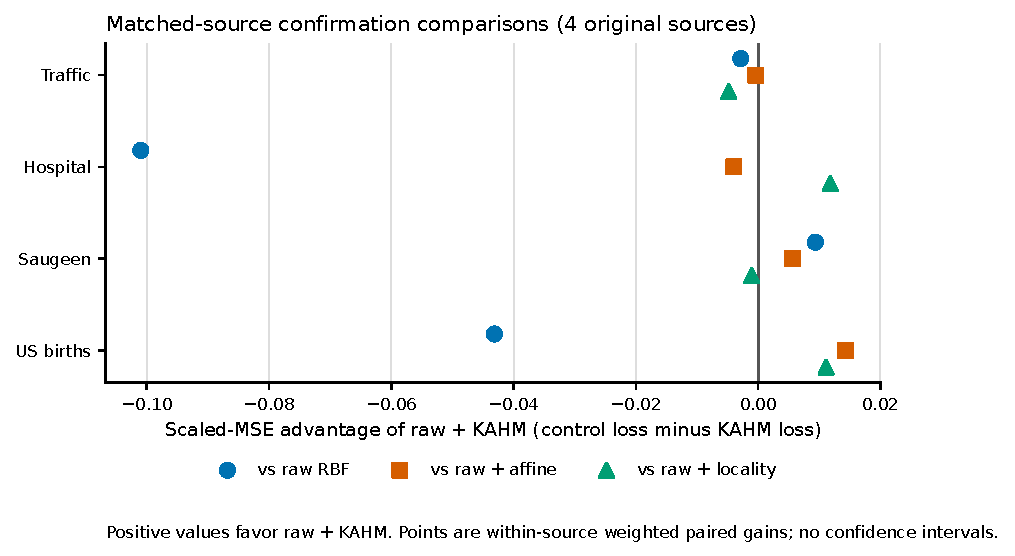
\includegraphics[width=\linewidth]{generated/figures/source_gains.pdf}
\caption{Within-source confirmation comparisons. Positive differences favor
raw-plus-KAHM. The plotted points are paired differences of the same
hierarchically weighted source means, not independent-window estimates.
The KAHM advantage over structural controls is small and changes sign
across sources.}\label{fig:source-gains}
\end{figure}

The raw-plus-affine and raw-plus-locality controls obtain 0.8458 and
0.8462, respectively. Raw-plus-KAHM improves on these aggregate values
by only 0.46\% and 0.50\%, with each comparison favoring KAHM in two
family means and the control in two. These small, mixed aggregate differences
do not establish that nonlinear reconstruction is the relevant mechanism.
The controls without
raw augmentation obtain losses 0.9449 for affine, 0.8964 for locality,
and 0.9354 for KAHM. Retaining the complete raw history helps the
aggregate performance of each local code here, but does not make the
augmented KAHM procedure superior to the raw-history baseline.

Capacity changes the magnitude of the result. At the small setting,
raw-plus-KAHM obtains 0.8551 versus raw RBF's 0.8383, about 2.00\% worse.
At the medium setting it obtains 0.8288 versus 0.7767, about 6.70\% worse.
Its small aggregate advantage over raw-plus-affine reverses at the medium
setting. The cap on training windows and the model sizes change together,
and the former binds only for the long confirmation series; this experiment
does not isolate their individual effects.

\subsection{Accuracy and complete measured computational cost}
Raw-plus-KAHM costs 0.3874 seconds per hierarchically weighted confirmation
task, compared with 0.1688 seconds for raw RBF, a factor of 2.30.
Raw ridge obtains lower mean loss than either at 0.1880 seconds. KAHM's
small aggregate improvements over raw-plus-affine and raw-plus-locality
come with 14.65\% and 38.82\% greater mean wall cost, respectively.
Figure~\ref{fig:accuracy-cost} plots these observed tradeoffs together
with the decision procedures. The measurements do not imply fixed
hardware-independent speed ratios, and individual source/capacity timings
can differ from the aggregate order.

Implementation overhead is material for these small fits. In particular,
selection cleanup, including explicit garbage collection, accounts for
0.1381 of raw RBF's 0.1688 seconds and 0.1825 of raw-plus-KAHM's
0.3874 seconds. Their search computations take 0.0130 and 0.1113 seconds,
and their final refits take 0.0051 and 0.0724 seconds, respectively.
The complete measured totals include this cleanup consistently. The
reported 2.30-fold ratio describes the supplied fitting workflow,
not an intrinsic arithmetic complexity ratio between feature maps.
Table~\ref{tab:cleanup-costs} separates cleanup and the launch-to-result
measurements for the matched pair.
\begin{table}[t]
\centering\small\setlength{\tabcolsep}{4pt}
\caption{Confirmation cost transparency for the primary matched pair, with equal source-family weighting. Total is the complete warm-library scientific pipeline. Cleanup is its measured selection-overhead component, including explicit garbage collection; the percentage is the ratio of aggregated component and total times. Launch separately reports the measured isolated-child launch-to-result interval. These are implementation-specific costs, not intrinsic kernel arithmetic or universal complexity ratios.}\label{tab:cleanup-costs}
\begin{tabular}{lrrrr}
\toprule
Method & Total (s) & Cleanup (s) & Cleanup (\%) & Launch (s) \\
\midrule
Raw RBF & 0.16879 & 0.13808 & 81.8 & 0.17748 \\
Raw + KAHM & 0.38741 & 0.18253 & 47.11 & 0.40097 \\
\bottomrule
\end{tabular}
\end{table}


\begin{figure}[t]
\centering
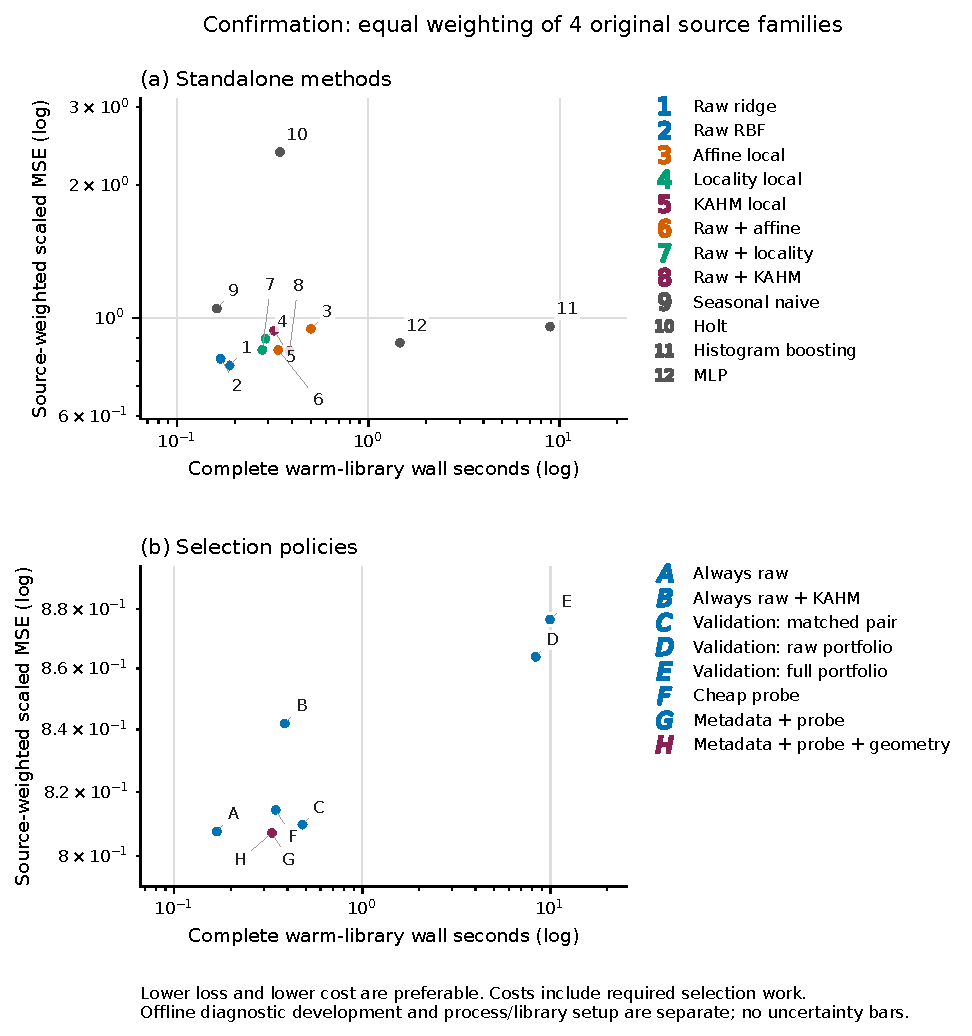
\includegraphics[width=\linewidth]{generated/figures/accuracy_cost.pdf}
\caption{Confirmation accuracy and warm-library scientific-pipeline cost.
All points use the same source hierarchy. The standalone and selector
panels have independently chosen scales to keep the full declared
comparisons visible. Selector costs include the searches and probes
needed to choose a model. No method is selected using the confirmation
outcomes for deployment.}\label{fig:accuracy-cost}
\end{figure}

The cost records include preprocessing, validation search with
within-method alpha-path reuse, final refitting, forecasting, and model
serialization. They separately expose the child launch-to-result interval
and library initialization. The two freeze processes recorded shared
library import costs of 8.724 and 4.873 seconds; these are distinct
measurements, not per-task charges or a claim that one method requires
every imported library. Across both phases, the sum of recorded task
intervals is 1,565.56 seconds (26.09 minutes), including every benchmarked
candidate, probe, orchestration, and prediction export. It excludes
unmeasured preparation intervals and pauses between stages.

Process high-water RSS averages 171.5 MiB for every standalone confirmation
method in this run. That common interpreter/input-dominated high-water
mark does not resolve incremental memory differences. Serialized model
sizes do differ: raw RBF averages 37.32 KiB, raw-plus-KAHM 179.2 KiB,
and raw ridge 5.655 KiB. A saved model's byte count should not be confused
with the memory needed to fit or query it.

The MLP baseline is also bounded by its declared iteration cap: 68 of
80 selected confirmation refits reach it. All such fits and warnings are
retained. No candidate exceeded the execution limits or was omitted.
The manuscript therefore compares the specified finite procedures;
it does not claim an optimally trained MLP or an optimized implementation
of every alternative.

\subsection{Does the frozen diagnostic identify useful KAHM cases?}
The primary increment, metadata-plus-probe-plus-geometry versus
metadata-plus-probe, changes none of the 80 confirmation decisions.
Both rules obtain scaled MSE 0.807085 and select raw-plus-KAHM on
31.25\% of the source-weighted task mass. Their mean warm-library costs
are both about 0.3309 seconds. The few microseconds separating their
recorded decision times have no practical interpretation. The geometric
features are already obtained from the paid KAHM probe, so this comparison
does not require an additional representation fit.

\begin{table}[t]
\centering\small\setlength{\tabcolsep}{4pt}
\caption{Frozen-policy confirmation outcomes over 4 source families with the same hierarchical weighting. Gain is raw-RBF scaled MSE minus chosen loss. Harm is the weighted fraction with loss more than 5\% above raw RBF. The final column counts selection of the specific raw-plus-KAHM pair member, including in portfolios. Wall cost includes all required probes/searches and decision inference, then the chosen final refit, forecast and model serialization. Offline evidence acquisition and diagnostic fitting are separate.}\label{tab:policy-summary}
\begin{tabular}{lrrrrr}
\toprule
Policy & Scaled MSE & Wall (s) & Gain & Harm (\%) & Raw+K (\%) \\
\midrule
Always raw & 0.8075 & 0.1688 & 0 & 0 & 0 \\
Always raw + KAHM & 0.8419 & 0.3874 & -0.0344 & 25 & 100 \\
Validation: matched pair & 0.8097 & 0.4812 & -0.002159 & 5.47 & 32 \\
Validation: raw portfolio & 0.8639 & 8.338 & -0.05638 & 10.9 & 0 \\
Validation: KAHM family & 0.8406 & 0.6242 & -0.03306 & 26.6 & 73.4 \\
Validation: full portfolio & 0.8764 & 9.948 & -0.0689 & 14.8 & 14.1 \\
Cheap probe & 0.8143 & 0.3465 & -0.006771 & 9.38 & 50 \\
Metadata & 0.816 & 0.2976 & -0.008445 & 15.6 & 50 \\
Metadata + geometry & 0.816 & 0.3695 & -0.008445 & 15.6 & 50 \\
Metadata + probe & 0.8071 & 0.3309 & 0.0004363 & 3.12 & 31.2 \\
Metadata + probe + geometry & 0.8071 & 0.3309 & 0.0004363 & 3.12 & 31.2 \\
\bottomrule
\end{tabular}
\end{table}


The identical decisions do not imply identical benefit estimates.
Log-benefit RMSE increases slightly, from 0.184549 without geometry to
0.184680 with it, and weighted sign accuracy is 58.59\% for both.
Always predicting that KAHM will not improve on raw has sign accuracy
61.72\% on these weighted confirmation tasks. This constant comparison
is descriptive and was not used to alter the frozen rule. Metadata-plus-
geometry also makes exactly the same choices as metadata alone, while
paying for its extra feature acquisition. Estimated-benefit errors and
fixed coefficients are reported in Appendix~\ref{app:full-results}.

\begin{figure}[t]
\centering
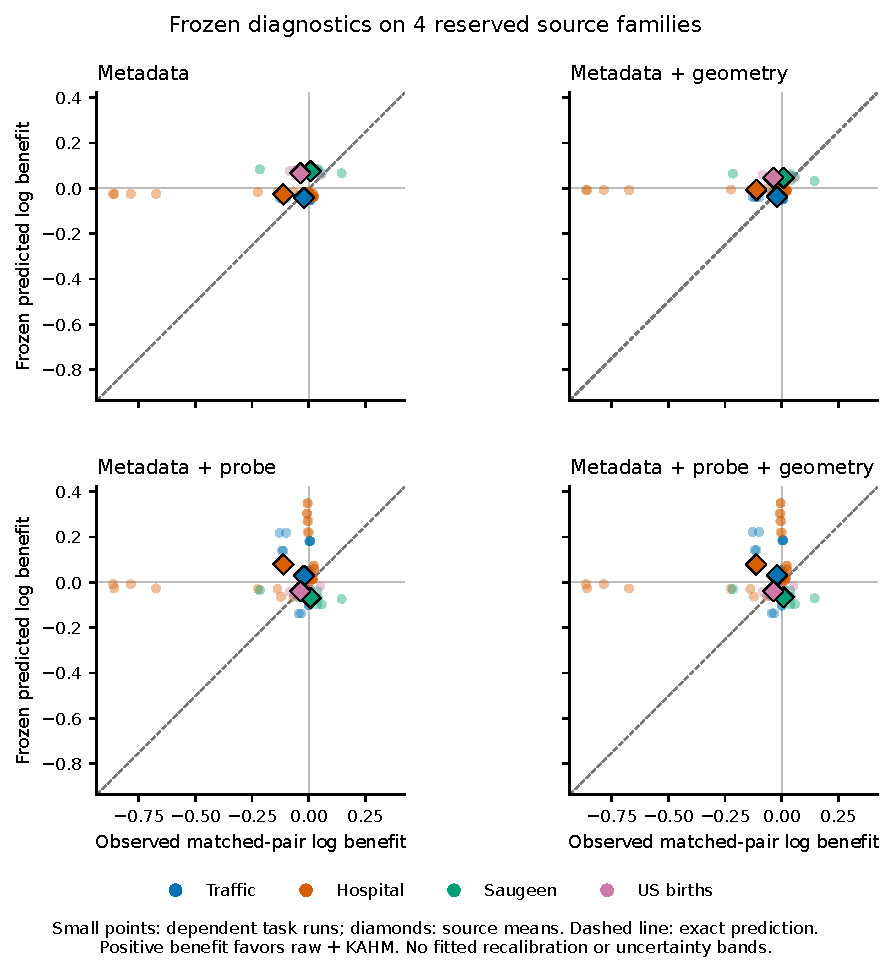
\includegraphics[width=0.92\linewidth]{generated/figures/diagnostic_predictions.pdf}
\caption{Observed versus frozen predicted log benefit for all four
diagnostics. Points within a source are dependent task runs; diamonds
show source means. Estimates are neither recalibrated on confirmation
data nor interpreted as probabilities. Similar selection decisions can
coexist with different estimated magnitudes.}\label{fig:diagnostic-predictions}
\end{figure}

The probe-based diagnostic's aggregate reduction from always-raw loss is
0.000436, or 0.054\%, at 1.96 times the raw predictor's pipeline cost.
It improves one source mean, worsens one, and ties two. It is better than
always choosing KAHM and better on these aggregates than the cheap-probe
decision or full validation portfolios. Those comparisons do not establish
the geometric increment or a practically useful gain over always raw.
The raw and full validation portfolios cost 8.338 and 9.948 seconds,
respectively, while obtaining losses 0.8639 and 0.8764. Counting every
candidate search prevents their choice of a comparatively inexpensive
final forecaster from concealing the cost of selection.

Offline learning is a separate investment. Acquiring the development
labels from the matched raw/KAHM pair costs a sum of 68.41 seconds of
standalone scientific-pipeline work. Adding the shared metadata/probe
dependencies gives 80.83 seconds; the four final diagnostic ridge fits
together add 0.032 seconds. These dependencies can be shared across
variants, so their separate acquisition totals must not be added.
The bookkeeping conservatively repeats preparation where cross-task
caching could be possible. Reporting only the millisecond-scale ridge
fits would substantially understate the measured cost of obtaining the
diagnostic. No invented number of future deployments is used to
amortize that investment.

\section{Discussion and limitations}\label{sec:discussion}
The three substantive questions have distinct answers in this bounded
study. Independent natural-source confirmation does not reproduce the
large development advantage over raw RBF. Complete measured costs make
the confirmed accuracy--cost comparison less favorable to raw-plus-KAHM,
while simpler raw ridge remains a strong alternative. Finally, the
specified geometric diagnostic increment supplies no improvement in
confirmation decisions beyond metadata and a paid validation probe.

These results are useful because the tests could have supported a
different conclusion. The frozen design retains conditional improvements,
including the small mean gain over raw RBF on Saugeen, as well as harms
and successful controls. It does not infer a universal failure from four
reserved families. The contribution is a reproducible examination of
where evidence for this particular KAHM forecasting procedure weakens:
a favorable development aggregate is concentrated, structural controls
explain much of the apparent benefit, and the proposed descriptors do
not yield a transferable adoption rule. A stronger claim about KAHM
would require further independent evidence, with a new confirmation
collection reserved before any new diagnostic is developed.


\subsection{What a representation comparison establishes}
Raw augmentation gives a clear information baseline: the original history
remains recoverable from the supplied code. A forecasting gain therefore
concerns the trained finite decoder and its regularization. It does not show
that KAHM has created additional target information. Conversely, a loss from
augmentation does not refute information preservation. Additional standardized
coordinates change distances, the finite Nystr\"om basis, and the effective
regularization geometry. These changes can make the prediction procedure
better or worse even though the raw coordinates remain present.

The affine and locality-aware augmentations are essential controls for this
reason. A favorable raw-versus-KAHM comparison by itself cannot attribute the
benefit to nonlinear KAHM reconstruction. Local coordinates, repeated views
of raw inputs, and their interaction with the downstream feature basis can
also matter. The declared alternatives share reference-selection rules and
have comparable local-coordinate constructions, while being fitted as
independent computational procedures. Actual feature widths and retained
Nystr\"om ranks are reported instead of assuming that the same landmark
count implies identical effective capacity.

\subsection{Limits of predicting benefit}
The diagnostic experiment concerns four specified, low-dimensional ridge
rules and one fixed reduced-capacity probe. A failure of those rules does
not establish that usefulness is unpredictable. A successful decision on
one family would likewise not establish a general adoption criterion.
With four development families, a complex learned selector would be hard
to validate independently; the present rules deliberately restrict their
flexibility and retain every prespecified variant.

Two design limits are especially relevant. The descriptors do not directly
encode the downstream landmark count. When the training-window cap does
not bind, the two capacity settings have identical diagnostic inputs even
though their full predictors differ. The history and horizon are also
changed together, so their individual effects cannot be identified by this
experiment. These are limitations of the evaluated criterion, and should
inform a future independently evaluated diagnostic rather than a retuning
of the reserved-source results.

Furthermore, predicting conditional mean log benefit is not the same
decision problem as minimizing conditional expected scaled MSE. Although
the sign of each realized log ratio agrees with the sign of its loss
difference, expectations of these quantities need not have the same sign
under heterogeneous losses. We therefore report both estimated-benefit
errors and the actual loss and cost of the resulting decisions. Input
geometry alone also cannot determine a universally preferable predictor:
different target relationships can be associated with the same input law.
The paid validation probe supplies target-relevant evidence, and the
geometric increment is evaluated against that information explicitly.

\subsection{Data, statistical scope, and computational scope}
The eight source families were deliberately selected from a public archive
for diversity and feasibility. They are not a probability sample of future
applications. Four families per phase support bounded descriptive comparisons;
series, horizons, capacity settings, seeds, and overlapping windows do not
increase that source count. We report family effects and sensitivity to
leaving out one family without attaching population confidence claims to
the small collection.

Some records are short. The longer Hospital and Traffic settings have only
21 and 29 training windows, respectively. NN5 T88 has seven available test
origins in the longer setting. The fixed roster retains this case, and its
loss estimates should be read with that limited support in mind. Missing
windows are excluded using the same availability rule for every method;
the resulting estimand concerns available complete windows, rather than
unobserved targets or operational forecasts with missing contexts. The
FRED-MD experiment is relative to a supplied retrospective snapshot and
cannot certify every upstream transformation or emulate real-time release
and revision constraints.

The comparison is restricted to local univariate forecasters, two small
capacity settings, and finite tuning grids. It includes a small MLP and
boosted-tree control but no global pretrained forecaster or comprehensive
state-of-the-art neural benchmark. The training-window cap is nonbinding
for the development sources and binding for the long confirmation series;
the larger setting therefore changes available sample count only for part
of the collection. The three-value alpha grid is fixed in advance, and a
boundary choice is not evidence that an optimum over all regularization
strengths has been located.

Measured costs apply to the supplied reference implementations on the
recorded CPU environment. Warm-library scientific-pipeline costs include
required feature construction, selection, refitting, prediction, and
serialization; library initialization and experimental process launch are
separate measurements. Timing small procedures can be sensitive to system
load and Python bookkeeping. The component records expose those effects.
Process high-water memory and serialized model size answer different
questions. The former includes the interpreter and input arrays and is
not an incremental memory estimate for a hypothetical combined selector.

\section{Conclusion}\label{sec:conclusion}
We evaluated KAHM-derived local features with independent natural-source
confirmation, explicit computational dependencies, and a prospectively
frozen usefulness diagnostic. The preserved synthetic study motivated
the experiment but was not counted as natural confirmation. On the four
reserved families, raw-plus-KAHM has higher aggregate error and cost
than the matched raw RBF predictor, and raw ridge has lower aggregate error than
either. Advantages over affine/locality augmentation are small and
source-dependent. Adding geometric features to metadata and a validation
probe changes no confirmation choices and provides no reduction in
log-benefit prediction error. The supplied artifacts preserve the
failures as well as improvements and independently reconstruct every
reported task--method loss. The evidence supports evaluating KAHM as
one conditional representation choice within a complete forecasting
procedure; it does not establish a broadly preferable predictor or a
validated rule for anticipating its benefit.



\section*{Reproducibility and author review}
The accompanying extension contains source snapshots, upstream dataset
attribution, configuration and dependency pins, two staged freeze records,
saved per-origin forecasts, cost nodes, and a one-command reconstruction of
the reported numbers and figures. The original source and outcome files are
checked against their checkpoint hashes. Numerical results were generated by
the disclosed programs; algorithmic assistance does not substitute for author
review. Final author contact information, funding declarations, and
competing-interest statements require author confirmation before submission.

\bibliography{references}
\appendix
\section{Relationship to the preserved manuscript}\label{app:checkpoint}
The previous manuscript, \emph{When Kernel Affine Hull Geometry Helps
Prediction: Local Coordinates, Decoder Capacity, and Conditional Gains},
is preserved with its reproducibility archive at commit
\texttt{a67c40190458bab7b3e56b4fac76770798d074b3}. The new extension records
SHA-256 hashes for all 217 previously tracked repository files and the seven
submission artifacts. The original study is neither relabeled as natural-data
confirmation nor pooled with the new source families. Its synthetic
experiments provide motivation and mechanism controls; the new confirmation
is based exclusively on the reserved natural sources.

At the 256-landmark setting, the earlier Van der Pol experiment reported mean
MSEs of 0.00165415 for raw inputs, 0.00107800 for affine local coordinates, and
0.00087197 for KAHM local coordinates. Across its separately defined capacity
contrast family, four comparisons supported practical benefit, six supported
harm, and two were unresolved. These are archived results, not newly estimated
effects or additional independent forecasting domains. The previous Airfoil
experiment was static regression and is not included as a natural forecasting
task in the present study.

The new implementation preserves the local KAHM definition while making
standalone alternative fitting and alpha-path reuse explicit. Its stable
Gaussian query calculation and raw-augmentation choices are specified in
Section~\ref{sec:nf-methods}. The former manuscript remains byte-identical;
the first-page disclosure in this new draft also addresses the placement
issue identified in the previous submission-format review.

\section{Reconstruction of the experiment}\label{app:reproduction}
The repository entry point is
\texttt{extensions/natural\_forecasting}. From the repository root, install
the extension's pinned requirements in Python 3.12, then run the synthetic
unit tests. The data command verifies the eight checksummed archive snapshots.
The experiment is separated into preparation, initial freeze, development,
diagnostic freeze, confirmation, and analysis:
\begin{verbatim}
python -m extensions.natural_forecasting.run prepare
python -m extensions.natural_forecasting.run initial-freeze
python -m extensions.natural_forecasting.run run --role development
python -m extensions.natural_forecasting.run freeze-confirmation
python -m extensions.natural_forecasting.run run --role confirmation
python -m extensions.natural_forecasting.run analyze
\end{verbatim}
Each command accepts a separate run directory. A new reproduction makes its
own freeze; the supplied reference freeze is immutable. Confirmation cannot
start without a matching code, dependency, roster, and diagnostic state.
Interrupted complete tasks can be resumed only when their prediction artifacts
match their recorded hashes. A failed task is retained and stops the run;
silently replacing a task or dropping a failed method is not permitted by the
analysis. The supplementary archive includes the exact reference results and
the metadata needed to audit them without refitting every predictor.

The two random seeds are 17 and 43. NumPy, SciPy, scikit-learn, statsmodels,
pandas, and threadpoolctl versions, thread settings, visible processor
information, and the separate library initialization cost are recorded in
the freeze. These details support reproducibility of the computation.
Wall-clock measurements remain specific to the declared shared CPU
environment, and process high-water memory is not an incremental allocation
measurement.

\begin{table}[t]
\centering\small\setlength{\tabcolsep}{4pt}
\caption{Completed experiment audit. Counts of forecasts, tasks and tests serve reproducibility checks; they do not increase the number of independent source families. The report builder reads existing predictions and validation evidence without rerunning forecasting or diagnostic inference.}\label{tab:validation-audit}
\begin{tabular}{lr}
\toprule
Audit item & Recorded result \\
\midrule
Final runner validation & passed \\
Development original source families & 4 \\
Confirmation original source families & 4 \\
Development / confirmation task runs & 128 / 80 \\
Total task runs & 208 \\
Saved candidate forecast arrays / dimensions checked & 2496 \\
Candidate losses independently recomputed by runner & 2496 \\
Targets and origins equal frozen source windows & True \\
Historical tracked files verified unchanged & 217 \\
Scientific protocol and both stage freezes intact & True \\
Unit tests in supplied evidence & 53 \\
\bottomrule
\end{tabular}
\end{table}


\section{Additional source and capacity results}\label{app:full-results}
All declared comparisons are retained below. The two context--horizon pairs
are coupled settings, so the tables do not separately identify a causal
context-length or horizon effect. Likewise, the two capacity settings change
both the cap on training windows and specified model sizes. Their timings are
observed costs rather than enforced equal-time budgets.
{\small\setlength{\tabcolsep}{4pt}
\begin{longtable}{lrrrrr}
\caption{Development scaled MSE by original source family. The final column gives equal-source aggregation; source columns retain the declared within-source weights. Development diagnostics use leave-one-source-family-out fits; confirmation diagnostics use the frozen development fit. Always-policy rows duplicate their corresponding standalone methods deliberately.}\label{tab:source-development-loss}\\
\toprule
Method or policy & FRED-MD & NN5 & Tourism & Electricity & Equal-source \\
\midrule
\endfirsthead
\toprule
Method or policy & FRED-MD & NN5 & Tourism & Electricity & Equal-source \\
\midrule
\endhead
Raw ridge & 0.5601 & 0.8584 & 2.865 & 0.4243 & 1.177 \\
Raw RBF & 10.46 & 0.7552 & 3.476 & 0.4388 & 3.783 \\
Affine local & 2.548 & 0.8795 & 3.769 & 0.4535 & 1.912 \\
Locality local & 23.83 & 0.8148 & 3.778 & 0.4112 & 7.209 \\
KAHM local & 12.23 & 0.9163 & 3.636 & 0.4525 & 4.309 \\
Raw + affine & 1.409 & 0.7614 & 3.172 & 0.4481 & 1.448 \\
Raw + locality & 10.18 & 0.7474 & 3.046 & 0.4418 & 3.603 \\
Raw + KAHM & 4.254 & 0.7704 & 3.229 & 0.4539 & 2.177 \\
Seasonal naive & 2.269 & 1.089 & 2.982 & 0.5507 & 1.723 \\
Holt & 0.2409 & 1.358 & 8.228 & 0.6984 & 2.631 \\
Histogram boosting & 34.02 & 0.8032 & 4.786 & 0.4404 & 10.01 \\
MLP & 1.022 & 0.8475 & 2.77 & 0.4715 & 1.278 \\
Always raw & 10.46 & 0.7552 & 3.476 & 0.4388 & 3.783 \\
Always raw + KAHM & 4.254 & 0.7704 & 3.229 & 0.4539 & 2.177 \\
Validation: matched pair & 5.267 & 0.7335 & 3.229 & 0.4415 & 2.418 \\
Validation: raw portfolio & 0.2409 & 0.8021 & 3.014 & 0.4528 & 1.127 \\
Validation: KAHM family & 4.104 & 0.7792 & 3.223 & 0.4572 & 2.141 \\
Validation: full portfolio & 0.2409 & 0.8052 & 3.092 & 0.4675 & 1.152 \\
Cheap probe & 5.106 & 0.742 & 3.25 & 0.4217 & 2.38 \\
Metadata & 4.254 & 0.7704 & 3.229 & 0.4539 & 2.177 \\
Metadata + geometry & 4.254 & 0.7704 & 3.394 & 0.4539 & 2.218 \\
Metadata + probe & 4.157 & 0.759 & 3.338 & 0.4342 & 2.172 \\
Metadata + probe + geometry & 4.215 & 0.7704 & 3.338 & 0.4342 & 2.189 \\
\bottomrule
\end{longtable}
}

{\small\setlength{\tabcolsep}{4pt}
\begin{longtable}{lrrrrr}
\caption{Development warm-library wall seconds by original source family. The final column gives equal-source aggregation; source columns retain the declared within-source weights. Development diagnostics use leave-one-source-family-out fits; confirmation diagnostics use the frozen development fit. Always-policy rows duplicate their corresponding standalone methods deliberately.}\label{tab:source-development-cost}\\
\toprule
Method or policy & FRED-MD & NN5 & Tourism & Electricity & Equal-source \\
\midrule
\endfirsthead
\toprule
Method or policy & FRED-MD & NN5 & Tourism & Electricity & Equal-source \\
\midrule
\endhead
Raw ridge & 0.3731 & 0.1631 & 0.1888 & 0.1873 & 0.2281 \\
Raw RBF & 0.1929 & 0.1912 & 0.1834 & 0.1692 & 0.1842 \\
Affine local & 0.3285 & 0.2805 & 0.2983 & 0.2863 & 0.2984 \\
Locality local & 0.5431 & 0.29 & 0.2784 & 0.2649 & 0.3441 \\
KAHM local & 0.3705 & 0.3696 & 0.3735 & 0.3369 & 0.3626 \\
Raw + affine & 0.2923 & 0.2998 & 0.2979 & 0.288 & 0.2945 \\
Raw + locality & 0.3185 & 0.2967 & 0.2988 & 0.2533 & 0.2918 \\
Raw + KAHM & 0.4275 & 0.3807 & 0.3252 & 0.3024 & 0.3589 \\
Seasonal naive & 0.2125 & 0.177 & 0.1834 & 0.1878 & 0.1902 \\
Holt & 0.3224 & 0.42 & 0.3682 & 0.316 & 0.3567 \\
Histogram boosting & 3.086 & 4.954 & 1.729 & 1.819 & 2.897 \\
MLP & 1.278 & 0.9551 & 0.8521 & 0.5508 & 0.9089 \\
Always raw & 0.1929 & 0.1912 & 0.1834 & 0.1692 & 0.1842 \\
Always raw + KAHM & 0.4275 & 0.3807 & 0.3252 & 0.3024 & 0.3589 \\
Validation: matched pair & 0.5562 & 0.5313 & 0.4929 & 0.4301 & 0.5026 \\
Validation: raw portfolio & 4.066 & 5.306 & 2.641 & 2.719 & 3.683 \\
Validation: KAHM family & 0.692 & 0.6568 & 0.6115 & 0.5511 & 0.6278 \\
Validation: full portfolio & 5.861 & 6.513 & 4.138 & 4.075 & 5.147 \\
Cheap probe & 0.4739 & 0.4615 & 0.4004 & 0.3328 & 0.4172 \\
Metadata & 0.4284 & 0.3815 & 0.3258 & 0.3031 & 0.3597 \\
Metadata + geometry & 0.5195 & 0.465 & 0.3474 & 0.3744 & 0.4266 \\
Metadata + probe & 0.5029 & 0.474 & 0.2891 & 0.3411 & 0.4018 \\
Metadata + probe + geometry & 0.5284 & 0.4828 & 0.2891 & 0.341 & 0.4103 \\
\bottomrule
\end{longtable}
}

{\small\setlength{\tabcolsep}{4pt}
\begin{longtable}{lrrrrr}
\caption{Confirmation scaled MSE by original source family. The final column gives equal-source aggregation; source columns retain the declared within-source weights. Development diagnostics use leave-one-source-family-out fits; confirmation diagnostics use the frozen development fit. Always-policy rows duplicate their corresponding standalone methods deliberately.}\label{tab:source-confirmation-loss}\\
\toprule
Method or policy & Traffic & Hospital & Saugeen & US births & Equal-source \\
\midrule
\endfirsthead
\toprule
Method or policy & Traffic & Hospital & Saugeen & US births & Equal-source \\
\midrule
\endhead
Raw ridge & 0.5737 & 0.8461 & 0.522 & 1.177 & 0.7798 \\
Raw RBF & 0.5739 & 0.8228 & 0.6106 & 1.223 & 0.8075 \\
Affine local & 0.5796 & 0.928 & 0.6462 & 1.626 & 0.9449 \\
Locality local & 0.5719 & 0.7702 & 0.6504 & 1.593 & 0.8964 \\
KAHM local & 0.5775 & 0.9029 & 0.6652 & 1.596 & 0.9354 \\
Raw + affine & 0.5764 & 0.9198 & 0.6068 & 1.28 & 0.8458 \\
Raw + locality & 0.572 & 0.9356 & 0.6002 & 1.277 & 0.8462 \\
Raw + KAHM & 0.5768 & 0.9238 & 0.6012 & 1.266 & 0.8419 \\
Seasonal naive & 0.6484 & 0.7848 & 1.023 & 1.743 & 1.05 \\
Holt & 0.6842 & 1.003 & 0.6079 & 7.197 & 2.373 \\
Histogram boosting & 0.6524 & 1.025 & 0.5386 & 1.606 & 0.9555 \\
MLP & 0.6811 & 1.15 & 0.5365 & 1.147 & 0.8785 \\
Always raw & 0.5739 & 0.8228 & 0.6106 & 1.223 & 0.8075 \\
Always raw + KAHM & 0.5768 & 0.9238 & 0.6012 & 1.266 & 0.8419 \\
Validation: matched pair & 0.5738 & 0.8236 & 0.6042 & 1.237 & 0.8097 \\
Validation: raw portfolio & 0.6087 & 1.116 & 0.5639 & 1.167 & 0.8639 \\
Validation: KAHM family & 0.577 & 0.9182 & 0.6012 & 1.266 & 0.8406 \\
Validation: full portfolio & 0.6122 & 1.099 & 0.5695 & 1.225 & 0.8764 \\
Cheap probe & 0.5761 & 0.8211 & 0.6253 & 1.235 & 0.8143 \\
Metadata & 0.5739 & 0.8228 & 0.6012 & 1.266 & 0.816 \\
Metadata + geometry & 0.5739 & 0.8228 & 0.6012 & 1.266 & 0.816 \\
Metadata + probe & 0.5761 & 0.8189 & 0.6106 & 1.223 & 0.8071 \\
Metadata + probe + geometry & 0.5761 & 0.8189 & 0.6106 & 1.223 & 0.8071 \\
\bottomrule
\end{longtable}
}

{\small\setlength{\tabcolsep}{4pt}
\begin{longtable}{lrrrrr}
\caption{Confirmation warm-library wall seconds by original source family. The final column gives equal-source aggregation; source columns retain the declared within-source weights. Development diagnostics use leave-one-source-family-out fits; confirmation diagnostics use the frozen development fit. Always-policy rows duplicate their corresponding standalone methods deliberately.}\label{tab:source-confirmation-cost}\\
\toprule
Method or policy & Traffic & Hospital & Saugeen & US births & Equal-source \\
\midrule
\endfirsthead
\toprule
Method or policy & Traffic & Hospital & Saugeen & US births & Equal-source \\
\midrule
\endhead
Raw ridge & 0.1454 & 0.1959 & 0.1905 & 0.2204 & 0.188 \\
Raw RBF & 0.1644 & 0.1636 & 0.1693 & 0.1779 & 0.1688 \\
Affine local & 0.2424 & 0.2732 & 0.4038 & 1.082 & 0.5002 \\
Locality local & 0.2311 & 0.254 & 0.4021 & 0.2721 & 0.2898 \\
KAHM local & 0.2579 & 0.2764 & 0.3496 & 0.4035 & 0.3218 \\
Raw + affine & 0.3969 & 0.2809 & 0.354 & 0.3199 & 0.3379 \\
Raw + locality & 0.2223 & 0.2752 & 0.3166 & 0.3022 & 0.2791 \\
Raw + KAHM & 0.2674 & 0.4235 & 0.4676 & 0.3911 & 0.3874 \\
Seasonal naive & 0.1551 & 0.164 & 0.1874 & 0.1393 & 0.1614 \\
Holt & 0.2759 & 0.3535 & 0.4118 & 0.3386 & 0.3449 \\
Histogram boosting & 1.774 & 1.39 & 17.59 & 14.89 & 8.91 \\
MLP & 0.4046 & 0.392 & 2.264 & 2.79 & 1.463 \\
Always raw & 0.1644 & 0.1636 & 0.1693 & 0.1779 & 0.1688 \\
Always raw + KAHM & 0.2674 & 0.4235 & 0.4676 & 0.3911 & 0.3874 \\
Validation: matched pair & 0.3909 & 0.5408 & 0.5273 & 0.4656 & 0.4812 \\
Validation: raw portfolio & 2.276 & 2.19 & 15.94 & 12.95 & 8.338 \\
Validation: KAHM family & 0.4622 & 0.6403 & 0.7116 & 0.6829 & 0.6242 \\
Validation: full portfolio & 3.595 & 3.661 & 17.63 & 14.9 & 9.948 \\
Cheap probe & 0.3029 & 0.2768 & 0.4534 & 0.3531 & 0.3465 \\
Metadata & 0.1651 & 0.1644 & 0.4686 & 0.3923 & 0.2976 \\
Metadata + geometry & 0.2216 & 0.2212 & 0.5797 & 0.4555 & 0.3695 \\
Metadata + probe & 0.2958 & 0.457 & 0.3033 & 0.2673 & 0.3309 \\
Metadata + probe + geometry & 0.2958 & 0.457 & 0.3033 & 0.2673 & 0.3309 \\
\bottomrule
\end{longtable}
}

{\small\setlength{\tabcolsep}{4pt}
\begin{longtable}{lrrrr}
\caption{Development capacity comparison. Each capacity changes specified training-window and model-size caps; it is not an equal-time budget. Values are equal-source weighted and retain all prescribed context--horizon settings and seeds.}\label{tab:capacity-development}\\
\toprule
Method or policy & medium MSE & medium wall (s) & small MSE & small wall (s) \\
\midrule
\endfirsthead
\toprule
Method or policy & medium MSE & medium wall (s) & small MSE & small wall (s) \\
\midrule
\endhead
Raw ridge & 1.177 & 0.28 & 1.177 & 0.1761 \\
Raw RBF & 4.582 & 0.1846 & 2.984 & 0.1838 \\
Affine local & 1.989 & 0.3292 & 1.836 & 0.2676 \\
Locality local & 8.238 & 0.4065 & 6.18 & 0.2817 \\
KAHM local & 3.855 & 0.3779 & 4.763 & 0.3473 \\
Raw + affine & 1.394 & 0.3071 & 1.501 & 0.282 \\
Raw + locality & 3.879 & 0.3038 & 3.327 & 0.2798 \\
Raw + KAHM & 2.332 & 0.3819 & 2.022 & 0.3359 \\
Seasonal naive & 1.723 & 0.2078 & 1.723 & 0.1725 \\
Holt & 2.631 & 0.345 & 2.632 & 0.3683 \\
Histogram boosting & 9.795 & 3.468 & 10.23 & 2.326 \\
MLP & 1.253 & 1.108 & 1.302 & 0.7098 \\
Always raw & 4.582 & 0.1846 & 2.984 & 0.1838 \\
Always raw + KAHM & 2.332 & 0.3819 & 2.022 & 0.3359 \\
Validation: matched pair & 2.342 & 0.5295 & 2.493 & 0.4758 \\
Validation: raw portfolio & 1.128 & 4.223 & 1.127 & 3.142 \\
Validation: KAHM family & 2.261 & 0.6594 & 2.021 & 0.5963 \\
Validation: full portfolio & 1.137 & 5.805 & 1.166 & 4.488 \\
Cheap probe & 2.297 & 0.4321 & 2.463 & 0.4022 \\
Metadata & 2.332 & 0.3828 & 2.022 & 0.3367 \\
Metadata + geometry & 2.364 & 0.4492 & 2.072 & 0.404 \\
Metadata + probe & 2.337 & 0.419 & 2.007 & 0.3846 \\
Metadata + probe + geometry & 2.348 & 0.4327 & 2.03 & 0.388 \\
\bottomrule
\end{longtable}
}

{\small\setlength{\tabcolsep}{4pt}
\begin{longtable}{lrrrr}
\caption{Confirmation capacity comparison. Each capacity changes specified training-window and model-size caps; it is not an equal-time budget. Values are equal-source weighted and retain all prescribed context--horizon settings and seeds.}\label{tab:capacity-confirmation}\\
\toprule
Method or policy & medium MSE & medium wall (s) & small MSE & small wall (s) \\
\midrule
\endfirsthead
\toprule
Method or policy & medium MSE & medium wall (s) & small MSE & small wall (s) \\
\midrule
\endhead
Raw ridge & 0.7635 & 0.1561 & 0.7961 & 0.2199 \\
Raw RBF & 0.7767 & 0.1719 & 0.8383 & 0.1657 \\
Affine local & 0.916 & 0.3088 & 0.9738 & 0.6917 \\
Locality local & 0.8908 & 0.3176 & 0.902 & 0.2621 \\
KAHM local & 0.9243 & 0.334 & 0.9466 & 0.3097 \\
Raw + affine & 0.8233 & 0.3859 & 0.8684 & 0.2899 \\
Raw + locality & 0.8363 & 0.2831 & 0.8561 & 0.275 \\
Raw + KAHM & 0.8288 & 0.3732 & 0.8551 & 0.4016 \\
Seasonal naive & 1.05 & 0.1621 & 1.05 & 0.1607 \\
Holt & 2.373 & 0.333 & 2.373 & 0.3569 \\
Histogram boosting & 0.9215 & 12.73 & 0.9896 & 5.086 \\
MLP & 0.8712 & 1.956 & 0.8859 & 0.9695 \\
Always raw & 0.7767 & 0.1719 & 0.8383 & 0.1657 \\
Always raw + KAHM & 0.8288 & 0.3732 & 0.8551 & 0.4016 \\
Validation: matched pair & 0.7847 & 0.4538 & 0.8347 & 0.5085 \\
Validation: raw portfolio & 0.8404 & 11.6 & 0.8874 & 5.074 \\
Validation: KAHM family & 0.8281 & 0.6116 & 0.8531 & 0.6369 \\
Validation: full portfolio & 0.8541 & 12.98 & 0.8987 & 6.918 \\
Cheap probe & 0.7943 & 0.3749 & 0.8343 & 0.3182 \\
Metadata & 0.8009 & 0.3187 & 0.8311 & 0.2764 \\
Metadata + geometry & 0.8009 & 0.3779 & 0.8311 & 0.3611 \\
Metadata + probe & 0.7765 & 0.2805 & 0.8377 & 0.3812 \\
Metadata + probe + geometry & 0.7765 & 0.2805 & 0.8377 & 0.3812 \\
\bottomrule
\end{longtable}
}

{\small\setlength{\tabcolsep}{4pt}
\begin{longtable}{lrrrr}
\caption{Estimated-benefit diagnostics with frozen hierarchical weights. These are descriptive log-benefit prediction errors and classification accuracies; they are not calibrated probabilities or interval coverage. No recalibration is fitted on confirmation data.}\label{tab:diagnostic-calibration}\\
\toprule
Diagnostic & Log RMSE & Log bias & Sign (\%) & 5\% class (\%) \\
\midrule
\endfirsthead
\toprule
Diagnostic & Log RMSE & Log bias & Sign (\%) & 5\% class (\%) \\
\midrule
\endhead
Development: Metadata & 1.035 & 0.01412 & 57 & 49.2 \\
Development: Metadata + geometry & 1.037 & 0.03491 & 47.7 & 43 \\
Development: Metadata + probe & 1.012 & 0.03064 & 52.3 & 53.9 \\
Development: Metadata + probe + geometry & 1.02 & 0.05091 & 50.8 & 43 \\
Confirmation: Metadata & 0.1643 & 0.05835 & 55.5 & 59.4 \\
Confirmation: Metadata + geometry & 0.1612 & 0.05269 & 55.5 & 75 \\
Confirmation: Metadata + probe & 0.1845 & 0.04069 & 58.6 & 73.4 \\
Confirmation: Metadata + probe + geometry & 0.1847 & 0.04196 & 58.6 & 71.9 \\
\bottomrule
\end{longtable}
}

{\small\setlength{\tabcolsep}{4pt}
\begin{longtable}{lrrrr}
\caption{One-off diagnostic development costs. Acquisition sums the union of both matched predictors' complete search/final nodes and each variant's metadata/probe/geometry dependencies within every development task. Summing standalone tasks can conservatively repeat preparation across seeds/tasks. Acquire and total denote wall time; CPU covers acquisition. Do not add the four rows: their developmental labels and some features can be shared. Ridge fitting is measured separately; no deployment-count amortization is assumed.}\label{tab:offline-costs}\\
\toprule
Variant & Acquire (s) & CPU (s) & Ridge (ms) & Total (s) \\
\midrule
\endfirsthead
\toprule
Variant & Acquire (s) & CPU (s) & Ridge (ms) & Total (s) \\
\midrule
\endhead
Metadata & 68.49 & 68.45 & 6.657 & 68.5 \\
Metadata + geometry & 78.6 & 78.56 & 10.04 & 78.61 \\
Metadata + probe & 80.83 & 80.79 & 9.035 & 80.84 \\
Metadata + probe + geometry & 80.83 & 80.79 & 6.146 & 80.84 \\
\bottomrule
\end{longtable}
}

{\small\setlength{\tabcolsep}{4pt}
\begin{longtable}{lrrrrrr}
\caption{Frozen development-only standardization and ridge coefficients, rounded for display. G denotes geometry and P the cheap probe. An absent feature is shown by a dash. Predictions use the unrounded values in the frozen diagnostic JSON and the fixed zero decision threshold.}\label{tab:diagnostic-coefficients}\\
\toprule
Feature & Mean & Scale & Meta & Meta+G & Meta+P & Meta+P+G \\
\midrule
\endfirsthead
\toprule
Feature & Mean & Scale & Meta & Meta+G & Meta+P & Meta+P+G \\
\midrule
\endhead
Intercept & -- & -- & 0.023966 & 0.023966 & 0.023966 & 0.023966 \\
log(1 + training windows) & 5.1417 & 0.66192 & 0.017096 & 0.013047 & -0.0099182 & -0.0089504 \\
log(1 + horizon/history) & 0.23442 & 0.019538 & -0.012299 & -0.013178 & -0.0043432 & -0.0045441 \\
Lag-one autocorrelation & 0.7189 & 0.24263 & 0.0069415 & 0.001093 & -0.014509 & -0.012806 \\
KAHM gate entropy & 0.074168 & 0.063288 & -- & -0.010312 & -- & -0.0026401 \\
log(1 + affine residual) & 0.18213 & 0.12986 & -- & -0.013232 & -- & 0.0063025 \\
Probe log-loss ratio & 0.25347 & 0.67921 & -- & -- & 0.14611 & 0.1467 \\
\bottomrule
\end{longtable}
}

{\small\setlength{\tabcolsep}{4pt}
\begin{longtable}{lrrrrr}
\caption{Recorded fitting behavior. Search and selected-refit warning events are separated. Counts describe task fits, which include dependent seeds and settings. Warned counts fits with recorded warnings; at cap counts selected refits reaching the recorded iteration limit. Full warning text is retained in the JSON report. No warning-triggered post hoc retuning is applied.}\label{tab:fit-warnings}\\
\toprule
Method & Fits & Warned & Search & Refit & At cap \\
\midrule
\endfirsthead
\toprule
Method & Fits & Warned & Search & Refit & At cap \\
\midrule
\endhead
Development: Raw ridge & 128 & 0 & 0 & 0 & 0 \\
Development: Raw RBF & 128 & 0 & 0 & 0 & 0 \\
Development: Affine local & 128 & 0 & 0 & 0 & 0 \\
Development: Locality local & 128 & 0 & 0 & 0 & 0 \\
Development: KAHM local & 128 & 0 & 0 & 0 & 0 \\
Development: Raw + affine & 128 & 0 & 0 & 0 & 0 \\
Development: Raw + locality & 128 & 0 & 0 & 0 & 0 \\
Development: Raw + KAHM & 128 & 0 & 0 & 0 & 0 \\
Development: Seasonal naive & 128 & 0 & 0 & 0 & 0 \\
Development: Holt & 128 & 0 & 0 & 0 & 0 \\
Development: Histogram boosting & 128 & 0 & 0 & 0 & 0 \\
Development: MLP & 128 & 128 & 232 & 105 & 105 \\
Confirmation: Raw ridge & 80 & 0 & 0 & 0 & 0 \\
Confirmation: Raw RBF & 80 & 0 & 0 & 0 & 0 \\
Confirmation: Affine local & 80 & 0 & 0 & 0 & 0 \\
Confirmation: Locality local & 80 & 0 & 0 & 0 & 0 \\
Confirmation: KAHM local & 80 & 0 & 0 & 0 & 0 \\
Confirmation: Raw + affine & 80 & 0 & 0 & 0 & 0 \\
Confirmation: Raw + locality & 80 & 0 & 0 & 0 & 0 \\
Confirmation: Raw + KAHM & 80 & 0 & 0 & 0 & 0 \\
Confirmation: Seasonal naive & 80 & 0 & 0 & 0 & 0 \\
Confirmation: Holt & 80 & 0 & 0 & 0 & 0 \\
Confirmation: Histogram boosting & 80 & 0 & 0 & 0 & 0 \\
Confirmation: MLP & 80 & 79 & 137 & 68 & 68 \\
\bottomrule
\end{longtable}
}

{\small\setlength{\tabcolsep}{4pt}
\begin{longtable}{lrrrrr}
\caption{Selection at numerical search-grid endpoints. Counts are descriptive; a two-point grid necessarily chooses an endpoint. These observations do not establish the benefit of a larger grid, and confirmation outcomes are not used to retune any method.}\label{tab:grid-boundaries}\\
\toprule
Method & Parameter & Choices & Lower & Upper & Declared grid \\
\midrule
\endfirsthead
\toprule
Method & Parameter & Choices & Lower & Upper & Declared grid \\
\midrule
\endhead
Development: Raw ridge & alpha & 128 & 84 & 4 & 0.01,1,100 \\
Development: Raw RBF & alpha & 128 & 35 & 4 & 0.01,1,100 \\
Development: Affine local & alpha & 128 & 45 & 8 & 0.01,1,100 \\
Development: Locality local & alpha & 128 & 35 & 9 & 0.01,1,100 \\
Development: KAHM local & alpha & 128 & 51 & 7 & 0.01,1,100 \\
Development: Raw + affine & alpha & 128 & 32 & 4 & 0.01,1,100 \\
Development: Raw + locality & alpha & 128 & 25 & 5 & 0.01,1,100 \\
Development: Raw + KAHM & alpha & 128 & 30 & 4 & 0.01,1,100 \\
Development: Histogram boosting & regularization & 128 & 78 & 50 & 0.01,1 \\
Development: MLP & regularization & 128 & 26 & 102 & 0.01,1 \\
Confirmation: Raw ridge & alpha & 80 & 20 & 56 & 0.01,1,100 \\
Confirmation: Raw RBF & alpha & 80 & 13 & 56 & 0.01,1,100 \\
Confirmation: Affine local & alpha & 80 & 9 & 58 & 0.01,1,100 \\
Confirmation: Locality local & alpha & 80 & 9 & 60 & 0.01,1,100 \\
Confirmation: KAHM local & alpha & 80 & 8 & 59 & 0.01,1,100 \\
Confirmation: Raw + affine & alpha & 80 & 12 & 59 & 0.01,1,100 \\
Confirmation: Raw + locality & alpha & 80 & 12 & 61 & 0.01,1,100 \\
Confirmation: Raw + KAHM & alpha & 80 & 12 & 60 & 0.01,1,100 \\
Confirmation: Histogram boosting & regularization & 80 & 34 & 46 & 0.01,1 \\
Confirmation: MLP & regularization & 80 & 5 & 75 & 0.01,1 \\
\bottomrule
\end{longtable}
}


\end{document}
